%====================================================================
%====================================================================
\section{Identifiability}
\frame{\frametitle{Outline} \tableofcontents[currentsection]}
%====================================================================
%====================================================================
\section{Extension to multivariate traits}
\frame{\frametitle{Outline} \tableofcontents[currentsection]}
%====================================================================
%====================================================================
\frame{\frametitle{Multivariate OU model}

  \paragraph{Data.} ${\bf X}_j = (X_{j1}, \dots X_{jp})$, possibly correlated (${\bf R}$).
  
  \bigskip \bigskip \pause
  \paragraph{Multivariate OU model ${\bf X}(t)$.} ${\bf W}(t) =$ standard multivariate BM:
  $$
  \dd {\bf X}(t) = {\bf A}(\text{\mathversion{bold}{$\beta$}} - {\bf X}(t)) \dd t + {\bf R} \; \dd {\bf W}(t)
  $$
  where $\bf{A} = \alpha \mathbf{I}$ \ra 'scalar' OU (scOU) model \refer{BAR17}.
  
  \bigskip \bigskip \pause
  \paragraph{Some comments.} 
  \begin{itemize}
%    \item Tractable inference if ${\bf A}$ and ${\bf R}$ commute.
   \item scOU: same 'recall' to the optimum for all traits (but arbitrary ${\bf R}$)
   \item $\ell1$ou \refer{KKR16}: arbitrary ${\bf A}$ but independent traits (${\bf R}$ diagonal)
   \item Preliminary pPCA \refer{Rev09} does not remove correlation \emphase{in presence of shifts}
   \item Preliminary de-correlation is still useful for numerical reasons
  \end{itemize}
}

%====================================================================
\frame{\frametitle{\url{PhylogeneticEM} package}

  \paragraph{Monkey dataset.}
  \begin{itemize}
  \item {\tt res <- PhyloEM(Y\_data = ..., phylo = ..., process = "scOU", K\_max = 10, nbr\_alpha = 4, ...)} 
  \item {\tt plot(res, ...)}
  \end{itemize}
  $$
  \includegraphics[height=.6\textheight]{../FIGURES/BAM17-SupMat-Fig2}
  $$
}

%====================================================================
\frame{\frametitle{\url{PhylogeneticEM} package}

  \paragraph{Monkey dataset.}
  \begin{itemize}
  \item {\tt eq\_shifts <- equivalent\_shifts(phylogeny, params\_5)} 
  \item {\tt plot(eq\_shifts, ...)}
  \end{itemize}
  
  $$
  \includegraphics[width=.9\textwidth]{../FIGURES/BAM17-SupMat-Fig3}
  $$
}

%====================================================================
\frame{\frametitle{Conclusion \& Future works}

  \paragraph{Conclusions.}
  \begin{itemize}
   \item Comprehensive estimation framework: EM algorithm + identifiability + model selection;
   \item JRSS-B paper: \refer{BMR16}
   \item Extension to correlated multivariate traits: \refer{BAR17}
   \item R package \url{Phylogenetic-EM}.
  \end{itemize}

  \bigskip \bigskip \pause
  \paragraph{Future work.}
  \begin{itemize}
%    \item 'Spasify' the multivariate version so that not all traits are affected by each shift;
   \item Deal with the uncertainty of the tree;
   \item Consider fossil records to distinguish between equivalent scenarios.
  \end{itemize}

}

%====================================================================
\frame[allowframebreaks]{ \frametitle{References}

\nocite{BMR16,BAR17}

{\tiny
  \bibliography{/home/robin/Biblio/BibGene}
%   \bibliographystyle{/home/robin/LATEX/Biblio/astats}
  \bibliographystyle{alpha}
  }
}

%====================================================================
\frame{\frametitle{Notations}
  
  $$
  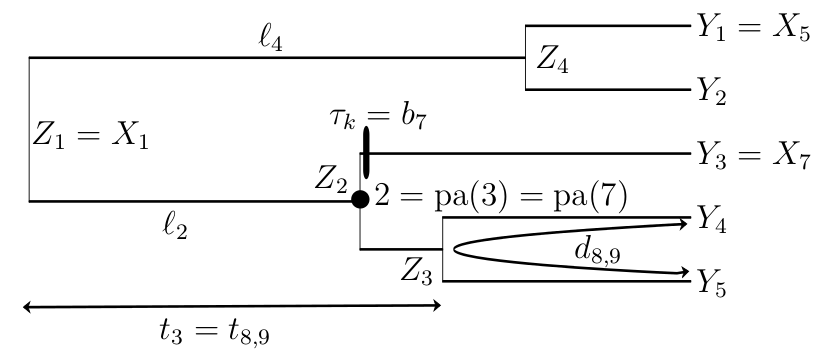
\includegraphics[width=.8\textwidth]{../FIGURES/Notations-BMR15}
  $$
  }
  
%====================================================================
%====================================================================
\end{document}
%====================================================================
%====================================================================

  \begin{tabular}{cc}
    \begin{tabular}{p{.5\textwidth}}
    \end{tabular}
    & 
    \hspace{-.02\textwidth}
    \begin{tabular}{p{.5\textwidth}}
    \end{tabular}
  \end{tabular}

